\documentclass[11pt]{article}

\usepackage[T1]{fontenc}
\usepackage[utf8]{inputenc}
\usepackage{charter}
\usepackage[scaled=0.9]{helvet}
\usepackage{courier}
\usepackage[margin=1in]{geometry}
\usepackage{microtype}
\usepackage{amsmath,amssymb}
\usepackage{booktabs}
\usepackage{tabularx}
\usepackage{longtable}
\usepackage{array}
\usepackage{enumitem}
\usepackage[dvipsnames]{xcolor}
\usepackage{tikz}
\usetikzlibrary{arrows.meta,positioning,calc,shapes.geometric,fit}
\usepackage{fancyvrb}
\usepackage[hidelinks]{hyperref}
\usepackage{titlesec}
\usepackage{caption}

\setlist{itemsep=2pt,topsep=4pt}
\setlength{\parskip}{4pt}
\setlength{\parindent}{0pt}
\setlength{\emergencystretch}{2.5em}
\renewcommand{\arraystretch}{1.18}
\captionsetup{font=small,labelfont=bf}

\usepackage{url}
\urlstyle{tt}
\makeatletter
\g@addto@macro{\UrlBreaks}{\do\_\do\:\do\-\do\,\do\/}
\makeatother
\newcommand{\code}{\path}
\newcolumntype{L}{>{\raggedright\arraybackslash}X}
\newcolumntype{P}[1]{>{\raggedright\arraybackslash}p{#1}}
\newcolumntype{R}[1]{>{\raggedleft\arraybackslash}p{#1}}

\definecolor{accent}{RGB}{176,58,46}
\definecolor{soft}{RGB}{245,240,236}
\definecolor{ok}{RGB}{39,110,72}

\newenvironment{keypoint}{\begin{center}
\begin{tikzpicture}\node[draw=accent,fill=soft,rounded corners=2pt,inner sep=8pt,text width=0.92\linewidth]\bgroup}{\egroup;\end{tikzpicture}\end{center}}

\title{\textbf{Breaking the Validator Stall Loop}\\[4pt]
\large Cost-accounted order-then-execute, built on the cost-accounting papers:\\ analysis, design, throughput model, and development plan}
\author{F1R3FLY.io --- design document, revision 3}
\date{October 28, 2026}

\begin{document}
\maketitle

\begin{center}
\small
\begin{tabular}{@{}lP{10.6cm}@{}}
\toprule
Repository & \code{F1R3FLY-io/f1r3node-rust} \\
Code basis & \code{integration/cost-accounted-ote-b1d866e45} at \code{d1f3ab5e1} (Oct 28, 2026), which carries Track~A and the B4 work through patch 0035 \\
Design basis & The cost-accounting papers in \code{F1R3FLY-io/publications} at \code{37915af} (Oct 28, 2026), read directly (\S\ref{sec:sources}) \\
Revision 3 & Rebuilds the cost-accounting design on the papers. Revision~2 took the papers second-hand from the branch's proposal and kept the branch's vault-based settlement. Adds a measured throughput model (\S\ref{sec:throughput}). The stall analysis, the consensus seam and the finalizer design of revision~2 stand. \\
Method & Code reading, and measurements on a 2-vCPU host (Intel Xeon at 2.1\,GHz, release build). Absolute times are host-specific. The ratios carry the argument. \\
\bottomrule
\end{tabular}
\end{center}

\begin{abstract}
\noindent Validators stall as they come under sustained load. The stall analysis of revisions 1 and~2 stands: a feedback loop through the finality lag, closed by two hard limits, with run-to-completion execution and the merge it forces at its root. Revision~3 changes the cost-accounting half of the design. The papers specify two things that the implementation does not yet do. First, payment is the consumption of a token in a communication, from a token stack located on the payer's own signature channel. Second, acceptance by a linear resource proof is itself the concurrency control, so that deploys with different signatures share no state and run concurrently. The implementation instead keeps money in the SystemVault, reads it through Rholang contracts, and settles every deploy through one shared vault contract after the run. Measured on the integration branch, settlement takes 83--94\,\% of block execution. A one-line deploy spends 1.2\,ms interpreting its term and about 675\,ms on funding and settlement. Settlement time per envelope also grows with block size, from 0.67\,s to 2.1\,s, which is the signature of a hot spot. This revision gives a design that follows the papers, a throughput model built from those measurements, and a revised plan. The model projects a 12--105-fold reduction of per-envelope work on the measured workloads, and near-linear scaling with cores for envelopes with independent signatures. Together these give two to three orders of magnitude over today's measured 0.44--1.24 envelopes per second for small deploys, and one to two orders for heavier ones. The model also identifies where these gains do not appear: payments that move REV through the SystemVault (7-fold), deploys dominated by their own computation, application-level hot channels, the consensus cap of envelopes per block, and multi-core RSpace efficiency, which is not yet measured.
\end{abstract}

\tableofcontents
\newpage

%======================================================================
\section{Summary}

\textbf{The stall.} Under sustained deploy load the unfinalized region of the DAG grows. Proposal preparation, merging, the deploy lifecycle register and the finality oracle all do work that grows with that region, which slows blocks and finality, which grows the region. Two limits turn the slowdown into a stop: a 15-second finalizer timeout that discards all work, and a merge cap at 256 blocks of floor distance (\S\ref{sec:analysis}). Track~A has delivered the fixes for the finality half of the loop on \code{dev}.

\textbf{The cause underneath.} Each deploy runs to completion against committed state, so concurrently produced blocks hold divergent post-states, and the node must merge them. The cost-accounting papers remove the reason for the merge: every interaction is gated by a token of the signatures involved, so potential conflicts are visible as shared signatures, and deploys can run at any time.

\textbf{The two central points of the design.} The papers make two promises, and this revision builds on both:
\begin{enumerate}
\item \textbf{No hot spots.} Each signer's tokens are a stack located on that signer's own channel. A deploy draws only on stacks that its own signatures name. Two deploys with different signatures touch disjoint state and cannot contend. A shared structure on the payment path would put every deploy on one causal chain, and that is exactly what the papers rule out.
\item \textbf{Concurrent deploys, little merge logic.} Acceptance by linear proof is the concurrency control. Competing deploys are competing proof obligations over the same linear hypotheses, and at most one succeeds before any step runs. Independent deploys then run concurrently. The only conflicts left are races on shared data channels, which the runner decides and records.
\end{enumerate}

\textbf{Where the implementation stands.} The consensus seam is largely in place: order-then-execute, structural validity, the linearizer, records, attestation, inclusion checks and pruning (patches 0028--0035). The funding path, however, departs from the papers. Money stays in the SystemVault as REV. Each deploy reads vault balances through Rholang (44.5\,ms per read) and, after its run, is settled by one vault contract that reserves, validates, apportions, burns, pays a shared fee vault and refunds. That play runs with an unlimited budget and writes about 1{,}000 events into the record. Every envelope's settlement touches the same vault map, fee vault and cost cursors, so settlements form one causal chain. The measured consequence: settlement is 83--94\,\% of block execution, and the branch executes 0.44--1.24 envelopes per second on the measurement host (\S\ref{sec:measured}).

\textbf{The design of this revision.} Payment becomes token consumption. An envelope's gate reads its signers' located stacks, not the vault. Its precharge moves the overestimate $\Delta^{\max}$ from those stacks into an escrow keyed by the envelope. Its run consumes the escrow, one token per COMM. Its refund returns the rest and moves the fee to the proposer's own fee channel. Each step touches only channels that the envelope's own signatures name. REV and tokens meet only at an explicit boundary, acquisition and redemption, which one vault operation serves for many deploys (\S\ref{sec:design}).

\textbf{Projected throughput.} On the measured workloads, per-envelope work falls 12- to 105-fold, and independent envelopes scale with cores. For one-line deploys the projection is about 190--280 envelopes per second on the 2-vCPU measurement host and 1{,}500--2{,}250 on 16 cores, against 0.44--1.24 today. Where gains are smaller, \S\ref{sec:limits} explains why, item by item.

\begin{keypoint}
\textbf{Decisions requested (\S\ref{sec:decisions}).}
\begin{enumerate}[label=(\arabic*),leftmargin=1.5em]
\item v6 settlement moves from the SystemVault to located token stacks, as the papers specify. The vault-based settlement and the precharge-and-refund design of October 28 are withdrawn.
\item REV and tokens meet only at acquisition and redemption.
\item The fee goes to the proposer's own fee channel, not to a shared fee vault.
\item Owners, sponsors and grants fund through located stacks and funding slots.
\item The throughput targets of \S\ref{sec:validation} become exit criteria for B3 and B7.
\end{enumerate}
\end{keypoint}

%======================================================================
\section{What revision 3 changes, and why}\label{sec:changes}

Revision~2 stated in its sources that it ``did not read the papers directly'', and took them as the branch's proposal quoted them. It got the signature-marking argument right: different signatures cannot conflict on funding, and agreement reduces to the race winners of each block and the order of conflicting blocks. It missed what the papers say about money. It does not mention token stacks. It adopted the branch's settlement as a library to port (``settle each envelope from its measured use; refund the remainder''). It kept the vault's contention patch as a requirement (``\code{SystemVault.rho} bucket locks (DR-119): Keep. Needed for concurrent settlement.''). It defined the record to include ``settlements, system work'', so the vault's event logs entered consensus.

The work of the last week traced each of these to a defect:
\begin{itemize}
\item \textbf{Record size.} Records came to about 100\,KB per envelope, 93\,\% logs, and 92\,KB of that was the vault settlement log. A block of more than about 80 envelopes produced a record that no block could carry, and the executor would stop (patch 0035).
\item \textbf{Unbounded system work.} Settlement runs with \code{Cost::unsafe_max()}. The gate's estimator cannot bound the vault contracts, whose channels are not fresh and whose recursion depends on received values (X2 and X6 of DR-122). System plays never draw on the meter at all: a test measured 0 phlo under any budget.
\item \textbf{The vault as a hot spot.} A precharge-and-refund design built on the vault, written October 28, measured worse than the code it replaced: 118\,KB per one-source send, with a fourth shared map added. That design is withdrawn.
\end{itemize}

Revision~3 therefore starts from the papers (\S\ref{sec:blueprint}), measures the gap (\S\ref{sec:measured}), and designs to close it (\S\ref{sec:design}). Everything in revision~2 that does not depend on the funding path stands: the stall analysis, the consensus seam, the canonical order, records and attestation, the finalizer design, backpressure, Track~A and the hook points.

%======================================================================
\section{The stall: analysis}\label{sec:analysis}

This section restates revision~2 in brief. The evidence and line references are unchanged, and Appendix~\ref{app:findings} lists the detailed findings.

\subsection{The core loop}

Under sustained load three quantities grow together: the pending deploy pool, the set of deploys included in blocks but not yet settled, and the unfinalized DAG cone. Each grows with the finality lag $D$, and each carries costs that scale with it (Figure~\ref{fig:loop}).

\begin{figure}[h]
\centering
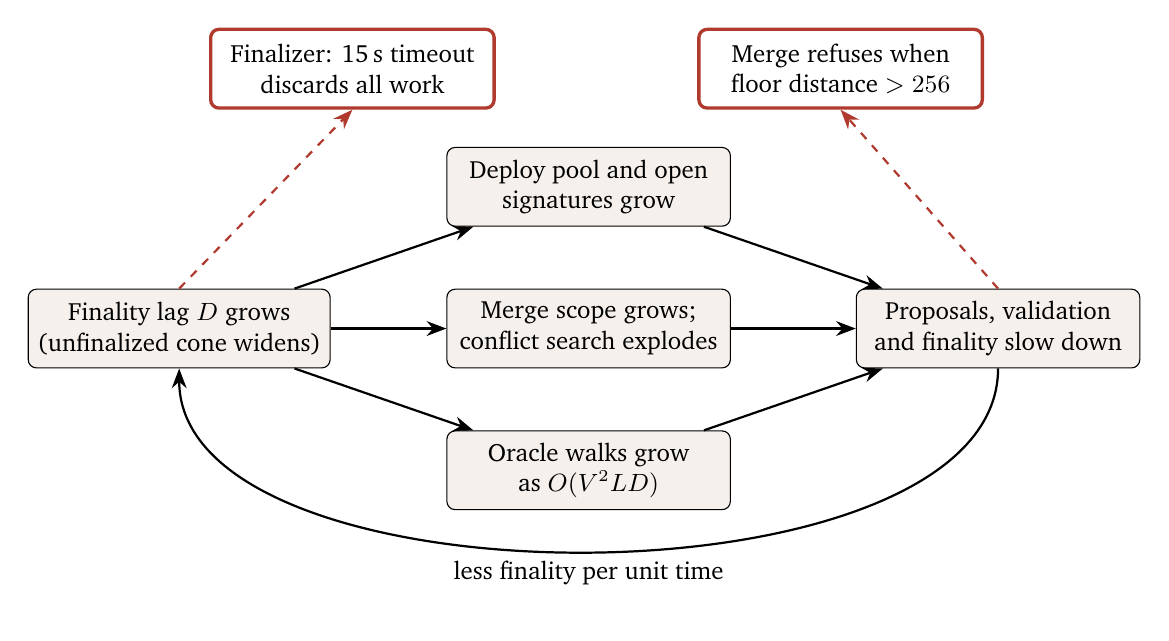
\begin{tikzpicture}[
  box/.style={draw,rounded corners=3pt,fill=soft,align=center,minimum width=3.6cm,minimum height=1.0cm,font=\small},
  trap/.style={draw=accent,very thick,rounded corners=3pt,fill=white,align=center,minimum width=3.6cm,minimum height=1.0cm,font=\small},
  arr/.style={-{Stealth[length=2.5mm]},thick}]
\node[box] (lag) at (0,0) {Finality lag $D$ grows\\(unfinalized cone widens)};
\node[box] (pool) at (5.2,1.8) {Deploy pool and open\\signatures grow};
\node[box] (merge) at (5.2,0) {Merge scope grows;\\conflict search explodes};
\node[box] (fin) at (5.2,-1.8) {Oracle walks grow\\as $O(V^2 L D)$};
\node[box] (slow) at (10.4,0) {Proposals, validation\\and finality slow down};
\draw[arr] (lag) -- (pool);
\draw[arr] (lag) -- (merge);
\draw[arr] (lag) -- (fin);
\draw[arr] (pool) -- (slow);
\draw[arr] (merge) -- (slow);
\draw[arr] (fin) -- (slow);
\draw[arr] (slow.south) .. controls (10.4,-3.6) and (0,-3.6) .. node[below,font=\small]{less finality per unit time} (lag.south);
\node[trap] (t1) at (2.2,3.3) {Finalizer: 15\,s timeout\\discards all work};
\node[trap] (t2) at (8.4,3.3) {Merge refuses when\\floor distance $>256$};
\draw[arr,accent,dashed] (lag.north) -- (t1.south);
\draw[arr,accent,dashed] (slow.north) -- (t2.south);
\end{tikzpicture}
\caption{The feedback loop. Every cost in the middle column grows with the finality lag. The two traps (outlined) turn the slowdown into a stop.}
\label{fig:loop}
\end{figure}

\subsection{Costs that grow with the lag, and the starvation paths}

\begin{itemize}
\item \textbf{Deploy pool.} About $8N$ signature checks per proposal for a pool of $N$, re-read under a lock.
\item \textbf{Lineage walks.} Quadratic in load: open signatures times segment length times deploys per block.
\item \textbf{Rejection-option search.} Exponential in conflicting pairs per group. Vault and PoS channels collapse groups into one, so the vault is a hot spot for the merge as well.
\item \textbf{Hot channels in RSpace.} $O(n)$ per touch and $O(n^2)$ over a run for a channel that accumulates $n$ datums. Replay scans its COMM list with a copy per step, $O(n^2)$ in COMMs (clone audit, finding~0.2).
\item \textbf{Finality walks.} $O(P \cdot V^2 L D)$ warm per block.
\item \textbf{Starvation.} A serial proposer queue, synchronous locks in async code, and CPU-bound consensus work on the async workers that also serve the network.
\end{itemize}

\subsection{Soak evidence}

The branch's proposal records two soaks. In August one merge call averaged 2.16\,s, 92\,\% of it settled-signature probes. In October no single stage separated failing sessions from passing ones, and the binding constraint had moved toward finality and Casper bookkeeping. The production high-phase replay targets recorded in \code{cost_accounting_perf_spec.rs} attribute about 229\,ms per deploy to precharge, 189\,ms to refund and 32\,ms to evaluation. That is, 93\,\% of replay time per deploy is spent moving money through the vault.

%======================================================================
\section{The blueprint: what the papers specify}\label{sec:blueprint}

This section reads the design from the papers. Each point ends with its consequence for the implementation.

\subsection{Signatures are names; token stacks are located terms}

The cost-accounted rho calculus extends names to $x, y ::= \lceil T \rceil \mid s$: signatures are channel names. Token stacks $S ::= () \mid s : S$ are first-class terms. Each layer is a balance cell of one signature. The companion paper refines the stack to a \emph{located} stack $S(I, s : S')$, a stack indexed by the surface $I$ that may draw on it. In rho this is a token stack sitting on a specific channel: only processes holding a matching channel name can consume from it. Unforgeable channels make that a genuine capability.

\emph{Consequence.} A signer's funds for computation are a stack on the signer's own channel in RSpace. They are not a balance in a shared contract.

\subsection{Payment is the communication}

The five rewrite rules are the COMM rule gated by token consumption. For a single signature,
\[
\{\, \mathtt{for}(y \leftarrow x)\,T \mid x!(U) \,\}_s \;\mid\; s : S \;\longrightarrow\; T\{\lceil U\rceil/y\} \;\mid\; S .
\]
The other four rules cover compound signatures and split or combined tokens. Joins follow one schema quantified over partitions, and conservation of authority holds across all of them: a join consumes exactly one receiver authority and one sender authority per channel.

\emph{Consequence.} The reducer charges by popping cells from located stacks. There is no separate settlement step that converts usage into money after the fact.

\subsection{Acceptance by linear proof is the concurrency control}

A deployment is accepted if and only if a linear proof of its resource use exists: for every signature $s$ it names, the supply $\Sigma_s$ meets the demand $\Delta_s$. The check runs before any step executes, and it is linear in the size of the AST. In the papers' words, two deployments competing for the same tokens are ``two proof obligations competing for the same linear hypotheses. At most one can succeed.'' Duplicate and simultaneous arrivals are resolved by the same rule, ``without locks, priority queues, or rollback mechanisms''.

\emph{Consequence.} Admission needs only the stacks of the envelope's own signers. Group decisions, later holds and shared cursors are unnecessary: committing tokens to an accepted deployment removes them from the supply that the next proof sees.

\subsection{Overcharge and refund}

Where control flow is data-dependent, the validator computes a conservative demand $\Delta^{\max}_c$, the maximum over reachable branches, and accepts if $\Sigma_c \ge \Delta^{\max}_c$. Execution consumes only the tokens it forces, and ``the residual $\Delta^{\max}_c - \kappa$ is returned to the client's token stack as part of the deployment's settlement''. The refund is safe because the number of tokens consumed equals the number of forced redexes, which the runtime counts exactly.

\emph{Consequence.} Settlement is a return of unused cells to the client's own stack. It is not a vault transaction.

\subsection{Located purses make the proof local}

Locating stacks decomposes the global resource obligation into one local linear proof per purse. The global proof is the separating conjunction of the local ones (companion paper, ``Local sufficiency composes''). Location also quarantines data-dependence to the surfaces that need a conservative bound.

\emph{Consequence.} The gate checks each signer's stack independently, and independent signers' checks can run concurrently.

\subsection{Chains and antichains: where hot spots come from}

The spacetime paper maps a cost-accounted computation to a measured causal set. Events are COMM firings, the order is enabling, and concurrency is Bernstein independence of footprints: no write-write and no read-write overlap. Two of its results bear directly on throughput:
\begin{itemize}
\item \textbf{Time from the stack.} The firings that draw on a single located stack form a chain, ordered by stack depth. A shared stack, or any shared resource that every deploy writes, serializes every deploy that touches it.
\item \textbf{Space from the surfaces.} Firings that draw on distinct stacks at non-near surfaces are concurrent: they form an antichain.
\item \textbf{Number is volume.} The phlogiston spent equals the number of events, and discrete proper time is the longest chain.
\end{itemize}
With $W$ the total work and $L$ the longest chain, a scheduler on $P$ cores completes the work in at most $W/P + L$ (Brent's bound). Throughput therefore depends on keeping $L$ short: no state that every deploy writes.

\emph{Consequence.} A design meets the papers' throughput promise only if nothing on the payment path is shared across signers. A shared vault map, fee vault or cursor puts every settlement on one chain, and $L$ grows with $W$.

\subsection{Fees, minting, sponsors and multi-signature}

\begin{itemize}
\item \textbf{Fees.} In the worked example, the validator handler takes one token from the client's address $A_c$ and keeps it on its own fee channel $F_v$. The fee lands on a per-validator channel.
\item \textbf{Minting.} Minting is constructing a token stack and sending it on a signature channel. Epoch phlogiston for validators, slush funds and fee-to-stake conversion use the same primitive.
\item \textbf{Funding slots.} A contract creates an unforgeable channel and lets any funder deposit tokens on it. This decouples who authorizes, who pays and what runs. A sponsor funds a new user through a slot.
\item \textbf{Multi-signature.} A compound signature $s_1 \otimes s_2$ needs tokens from every component. Weakening is forbidden, so a compound token must be spent in full or explicitly split.
\end{itemize}

\emph{Consequence.} Sponsors, grants and owners are funding slots and located stacks, not post-run vault debits.

\subsection{Internalisation}

The papers give a source-to-source translation of the cost-accounted calculus into pure Rholang~1.1, with splitter and joiner infrastructure. This gives cost-accounted semantics on today's runtime while the native implementation is built. The history-and-cost note adds that such an internalisation is lax: it carries an overhead grade. The native implementation is therefore the throughput path, and the translation is a bridge.

%======================================================================
\section{The gap, measured}\label{sec:measured}

\subsection{How the funding path works today}

The branch already has the papers' mechanism, but the v6 path does not use it:
\begin{itemize}
\item \textbf{Located stacks exist.} The reducer evaluates a token stack term by producing a \code{CostStack} datum on the signature channel of its head cell (\code{reduce.rs}, \code{eval_cost_stack}). The supply module models purse stacks and their inventory (\code{costacc/supply.rs}). Stack pops are accounted natively (\code{accounting/authority.rs}, \code{stack_pops}).
\item \textbf{v6 offers bypass them.} An owner-direct offer funds ``every class of the signer's own principal lane'' from the signer's vault (\code{owner_offer.rs}). The gate's supply ``counts SystemVault balances only'' (\code{gate.rs}). Fresh usage is bought from REV at the signed price on every deploy.
\end{itemize}

\begin{longtable}{@{}P{4.4cm}P{5.2cm}P{5.4cm}@{}}
\toprule
\textbf{Blueprint} & \textbf{Implementation (v6 path)} & \textbf{Measured effect} \\
\midrule
\endhead
Supply is the depth of the signer's located stack. & Supply is read from SystemVault balances through Rholang queries. & 44.5\,ms per balance query. The run phase spends 110--160\,ms beyond interpreting the term. \\
Payment is the COMM popping a cell. & The run is metered natively. The charge is then converted to REV and settled by \code{applyPhloCost}. & 560--600\,ms and about 1{,}000 events per envelope, under \code{Cost::unsafe_max()}. \\
Refund returns $\Delta^{\max} - \kappa$ to the client's stack. & \code{reserveAll}, \code{validateSettlement} and \code{settleReserved} run together after the run. & The reserve-and-refund happens, collapsed into one play after the run. \\
The linear proof is the concurrency control. & Holds that move no funds, plus \code{decide_groups}, \code{LaterHolds}, a held-capacity guard and the DR-28 cursors. & Settlement runs sequentially in block order. \\
The fee goes to the validator's own channel. & One fee vault, reached through \code{findOrCreate} by every settlement. & One write target shared by every envelope. \\
Distinct signers form an antichain. & Every settlement touches the vault map, the fee vault and the cursor map. & Settlement time per envelope grows with block size (Table~\ref{tab:blocks}). \\
The record carries the COMM log with charges. & The record also carries the wallet and receipt logs of the vault contracts. & About 92\,KB of a 100\,KB entry. \\
\bottomrule
\end{longtable}

\subsection{Measurements}

All figures come from release builds on the 2-vCPU host named on the first page, using tests in \code{casper/tests/v6_executor_spec.rs} and \code{casper/tests/util/rholang/cost_accounting_perf_spec.rs}.

\begin{table}[h]
\centering\small
\begin{tabular}{@{}rrrrrr@{}}
\toprule
\textbf{Envelopes} & \textbf{Runs} & \textbf{Settlement} & \textbf{Settlement share} & \textbf{Settlement per envelope} & \textbf{Envelopes/s} \\
\midrule
1 & 0.14\,s & 0.67\,s & 83\,\% & 0.67\,s & 1.24 \\
4 & 0.51\,s & 2.73\,s & 84\,\% & 0.68\,s & 1.24 \\
16 & 1.84\,s & 14.2\,s & 88\,\% & 0.89\,s & 1.00 \\
64 & 8.13\,s & 136.6\,s & 94\,\% & 2.14\,s & 0.44 \\
\bottomrule
\end{tabular}
\caption[Block execution by block size]{Block execution on the integration branch by block size (one-line sends from distinct payers; \code{phase_timings_by_block_size}). Settlement per envelope grows with block size, which is the mark of shared state.}
\label{tab:blocks}
\end{table}

\begin{table}[h]
\centering\small
\begin{tabular}{@{}lrrrr@{}}
\toprule
\textbf{Workload (one envelope)} & \textbf{Interpret term} & \textbf{v6 run phase} & \textbf{v6 settlement} & \textbf{Useful share} \\
\midrule
One send & 1.2\,ms & 112\,ms & 563\,ms & 0.17\,\% \\
256 sends & 29.7\,ms & 192\,ms & 605\,ms & 3.7\,\% \\
300 recursive COMMs & 32.5\,ms & 184\,ms & 572\,ms & 4.3\,\% \\
128 COMMs carrying 1\,KB each & 52.3\,ms & 211\,ms & 602\,ms & 6.4\,\% \\
REV transfer through the SystemVault & 81.6\,ms & --- & --- & --- \\
\bottomrule
\end{tabular}
\caption[Where the time of one envelope goes]{Where the time of one envelope goes (\code{cost_breakdown_of_one_envelope}, \code{a_user_vault_transfer_costs}). ``Interpret term'' is an unmetered exploratory run of the same term. Spawning a runtime costs 3.6\,ms and is subtracted.}
\label{tab:breakdown}
\end{table}

\textbf{Legacy \code{dev} pays the same cost.} The legacy precharge and refund system deploys, which also move REV through the vault, take 364\,ms and 291\,ms per deploy on the play path, against 0.3\,ms of evaluation. On replay, a block of seven deploys spends 106\,ms on precharge, 70\,ms on refund and 0.5\,ms on evaluation per deploy. The vault-centred payment path is the dominant per-deploy cost on both the legacy and the v6 path.

\textbf{System work is invisible to the meter.} The vault plays measured on October 28 report 0 phlo used under any budget. Work under the system signature is never drawn from a budget, so no allowance can bound it. Its event count is deterministic and linear in the number of sources: about 157 events (16\,KB) per source per play.

%======================================================================
\section{Design: cost-accounted order-then-execute on token stacks}\label{sec:design}

\subsection{Principles}

\begin{enumerate}[label=P\arabic*.,leftmargin=2.2em]
\item \textbf{Payment is consumption.} The reducer pays for a COMM by popping a cell from a located stack. Nothing converts usage into money after the run.
\item \textbf{No shared state on a deploy's payment path.} Everything that a deploy reads or writes to pay for itself is named by its own signatures: its stacks, its funding slots, its escrow. The single exception is the proposer's fee channel, which is per validator.
\item \textbf{Money and tokens meet at a boundary.} Acquisition turns REV into cells, and redemption turns cells back into REV. Each is one explicit vault operation, and it serves many deploys.
\item \textbf{Concurrency from independence.} Envelopes whose footprints are Bernstein-independent run concurrently. Conflicts are races on shared data channels, decided by the runner and recorded.
\item \textbf{The consensus seam stays.} Order-then-execute, structural validity, the linearizer, records, attestation, inclusion checks, the finalizer design and backpressure are those of revision~2, as delivered in patches 0028--0035.
\end{enumerate}

\subsection{The life of an envelope}

\begin{Verbatim}[fontsize=\footnotesize,frame=single,framesep=6pt]
gate(e, R):                         -- at the block pre-state, before any step
  for each signature s that e names:
    Delta_s = linear demand of e for s  (Delta_max where data-dependent)
    Sigma_s = depth of the located stacks of s at R  (native read)
  accept iff Sigma_s >= Delta_s + fee_s for every s  (one proof per purse)
precharge(e):                       -- in block order
  move Delta_s + fee_s cells from the stacks of s into escrow(e)  (native)
  a stack is short (an earlier envelope drew on it): reject e, no change
run(e):                             -- concurrent with the other envelopes
  each COMM pops cells from escrow(e) under rules 1-5 and the join schema
refund(e):                          -- in block order, after the merge
  fee cells -> fee channel of sender(block)
  unconsumed cells -> the stacks they came from
  exhausted (signed-limit bound reached): keep the whole precharge
\end{Verbatim}

\begin{itemize}
\item \textbf{Native, not Rholang.} The gate's supply read, the precharge, the refund and the fee transfer are RSpace operations on signature channels, done by the runtime. They run no contract code and have no Rholang event log. Their cost is a few produce and consume operations per signer.
\item \textbf{The escrow is the reservation.} Cells in escrow are no longer in the signer's stack, so a later envelope's gate sees the reduced supply. Duplicate and simultaneous arrivals behave as the papers describe.
\item \textbf{The meter is the stack.} The run's budget is the escrow. ``Out of phlogiston'' means the escrow is empty.
\item \textbf{Exhaustion.} Under a signed-limit bound, exhaustion rolls back the run's state and keeps the whole precharge, as \code{dev} does and as D-12 preserved.
\end{itemize}

\subsection{Acquisition and redemption}

A signer whose stack is short acquires cells with REV. Acquisition is one vault debit (REV, at the signed \code{phloPrice}) and one mint of cells onto the signer's stack. It runs either as a separate envelope or as the first action of an envelope whose gate finds the stack short. In both cases it is one vault operation for a batch of cells chosen by the client, so its cost is amortized across many deploys. Redemption is the reverse. The REV value of a cell is fixed at acquisition: a unit of account, as the virtual-token note puts it, not a per-deploy settlement.

\emph{Relation to D-12.} D-12 requires \code{phloLimit} and \code{phloPrice} on every deploy, with prepayment, refund, exhaustion and the minimum-price check. Under this design \code{phloLimit} bounds $\Delta$, the cells an envelope may precharge. \code{phloPrice} is the price of any acquisition the envelope performs, and the minimum-price check applies to it. Prepayment is the precharge, the refund is the return of unused cells, and exhaustion keeps the precharge. This mapping needs ratification as the ``separate normative mapping'' D-12 asked for (Q-13).

\subsection{Owners, sponsors and grants}

\begin{itemize}
\item \textbf{Owners} (DR-135) pay for the regions of their stored processes at their own price. Under this design an owner keeps a located stack, and an owner region pops from it as its COMMs fire. No debit follows the run. An owner without cells refuses the introduction, as the branch's region refusal already does.
\item \textbf{Sponsors} use funding slots: an unforgeable channel with deposited cells, named by the deploy that it funds.
\item \textbf{Grants} are funding slots with a validity window that the gate checks at block time.
\end{itemize}

\subsection{Block execution}

\begin{enumerate}
\item \textbf{Gate} every envelope at $R_0$. The checks are independent per signer and run concurrently.
\item \textbf{Precharge} in block order, natively. Envelopes that share a signer are serialized here by their stacks, exactly as the linear proof prescribes. Different signers' precharges touch different channels.
\item \textbf{Run} every admitted envelope concurrently from the precharged root.
\item \textbf{Merge} in block order. A conflicting envelope is rolled back and keeps its charge for the run, as decided on October 25.
\item \textbf{Refund} and pay fees in block order, natively.
\end{enumerate}
The ordered steps (2 and 5) are cheap native operations. The expensive step, the run, is the concurrent one.

\subsection{Records}

A record entry carries the gate verdict, the outcome, the cells drawn and returned per signature, the budget recording and operation journal needed for replay, and the user COMM log. It carries no system log. With the 0035a analysis of 1.25 bytes of user log per phlo (0.1 measured), an entry is at most $1.25\,\Delta + r_0$ bytes, with $r_0$ under 4\,KB measured. A per-block demand cap $D$ with $1.25\,D + E\,r_0 \le$ \code{block-record-bytes} then guarantees that every record can be cited. That closes the liveness hole of 0035 by arithmetic alone, and citing records in pieces (0035b) is no longer needed.

\subsection{What leaves the v6 path}

\begin{itemize}
\item The SystemVault settlement call \code{applyPhloCost}, its unlimited budget, and its logs in the record.
\item Vault reads in the gate. Supply becomes a stack depth.
\item Holds as fit checks, \code{decide_groups}, \code{LaterHolds} and the held-capacity guard.
\item The DR-28 monetary cursors and their vault validation, and with them the reason for the DR-119 bucket locks.
\item The shared fee vault.
\item The vault-based precharge and refund of October 28 (withdrawn before merge).
\end{itemize}
All of these stay on legacy shards, which remain byte-identical to \code{dev}.

\subsection{The consensus seam (unchanged from revision~2)}

The following stand as designed in revision~2 and delivered in patches 0028--0035:
\begin{itemize}
\item \textbf{Block content and validity.} Accepted envelopes without event logs, an attestation $(E, r_E)$, cited records, and structural validity that runs no Rholang and replays nothing.
\item \textbf{Canonical order.} Epochs along the main chain, a topological sort with fixed tie-breaks, and A-LIN checked by the linearizer and at commit.
\item \textbf{Executor, records and attestation.} One runner, verified replay, canonical records, attestation checks and evidence.
\item \textbf{Pruning, lag gate and pacing.} Patches 0030, 0032 and 0035.
\item \textbf{Charge model.} Charges as functions of events, operations named by source and occurrence, recorded interleaving decisions, concurrent replay with a bounded verdict (B2).
\item \textbf{Finalizer.} Compute, Validate and Commit (A1a--A1c).
\item \textbf{Epochs and slashing.} Bonds from attested state with an epoch lag (B6).
\end{itemize}

%======================================================================
\section{Throughput analysis}\label{sec:throughput}

\subsection{Model}

Let an envelope's core time be the sum of four parts: its interpretation $u$, the metering overhead factor $m$ on that interpretation, its funding work $f$ (gate, precharge, refund, fee), and its share $c$ of the block's checkpoint and merge. On $P$ cores with parallel efficiency $\eta$, and with the longest chain $L$ short relative to the work, node throughput is
\[
X \;\approx\; \frac{\eta\,P}{m\,u + f + c}.
\]
Every validator executes or replays every block, so shard throughput equals the throughput of one node. Adding validators adds safety, not throughput.

\textbf{Today.} $f$ is the run-phase funding overhead (110--160\,ms) plus settlement (560--600\,ms), and settlement is one chain. The parallel term does not apply to it, and its per-envelope cost grows with block size.

\textbf{Design.} $m = 1.2$, from the branch's own profiles (15--23\,\% more CPU in the reducer). The funding work $f$ covers a native stack read per signer, one escrow move each way, a fee move and the gate's linear estimate. The checkpoint share is $c \approx 0.5$\,ms (31\,ms per 64-envelope block measured). Together $f + c$ is taken as 2 to 8\,ms, with 5\,ms as the middle value, so an envelope costs $m\,u + 5$\,ms. That range is an estimate until S1 measures it.

\subsection{Per-envelope work}

\begin{table}[h]
\centering\small
\begin{tabular}{@{}lrrrr@{}}
\toprule
\textbf{Workload} & \textbf{Today} & \textbf{Design (range)} & \textbf{Gain, middle} & \textbf{Gain, range} \\
\midrule
One send & 675\,ms & 6.4\,ms (3.4--9.4) & 105$\times$ & 72--198$\times$ \\
256 sends & 796\,ms & 40.6\,ms (37.6--43.6) & 20$\times$ & 18--21$\times$ \\
300 recursive COMMs & 756\,ms & 44.0\,ms (41.0--47.0) & 17$\times$ & 16--18$\times$ \\
128 COMMs carrying 1\,KB & 813\,ms & 67.8\,ms (64.8--70.8) & 12$\times$ & 11--13$\times$ \\
REV transfer through the vault & 756\,ms & 103\,ms & 7.3$\times$ & --- \\
\bottomrule
\end{tabular}
\caption{Core time per envelope, today (run phase plus settlement, single-envelope block) and projected. The gain is largest where the deploy does least, because today's cost is almost all fixed funding overhead.}
\label{tab:gain}
\end{table}

\subsection{Node throughput}

\begin{table}[h]
\centering\small
\begin{tabular}{@{}lrrrr@{}}
\toprule
\textbf{Workload} & \textbf{2 cores} & \textbf{8 cores} & \textbf{16 cores} & \textbf{32 cores} \\
\midrule
One send & 187--281 & 750--1{,}124 & 1{,}499--2{,}249 & 2{,}998--4{,}497 \\
256 sends & 30--44 & 118--177 & 236--354 & 472--709 \\
300 recursive COMMs & 27--41 & 109--164 & 218--327 & 436--655 \\
128 COMMs carrying 1\,KB & 18--27 & 71--106 & 142--213 & 283--425 \\
REV transfer through the vault & 12--17 & 47--70 & 93--140 & 187--280 \\
\bottomrule
\end{tabular}
\caption{Projected envelopes per second for one node, with parallel efficiency $\eta$ from 0.6 to 0.9, for envelopes with independent signers and no shared data channel. Today's measured rate on the same 2-core host is 0.44 (64-envelope blocks) to 1.24 (single-envelope blocks). Absolute values are for the measurement host. Faster hosts scale all figures alike, today's included.}
\label{tab:throughput}
\end{table}

\textbf{Reading the tables.} On 2 cores, the design projects 150--640 times today's measured rate for one-line deploys (against 1.24 envelopes per second for single-envelope blocks and 0.44 for 64-envelope blocks). For the heavier workloads it projects 14--36 times their single-envelope rate of 1.2--1.3 per second. On 16 cores, with independent signers, the factors become about 1{,}200--5{,}100 and 110--290. The gain has two sources that multiply: removing fixed funding overhead (Table~\ref{tab:gain}) and replacing one causal chain with an antichain, so that cores apply (Table~\ref{tab:throughput}).



\subsection{Where the anticipated gains do not appear}\label{sec:limits}

The model supports large gains for overhead and concurrency. It does not support them unconditionally. These are the cases where it projects less, and why.

\begin{enumerate}
\item \textbf{Payments that move REV through the SystemVault.} A REV transfer is itself 81.6\,ms of vault contract code: registry lookup, tree-map lookups, auth key check, purse split and deposit. Removing settlement removes 675\,ms of overhead but leaves the transfer. The gain is 7.3 times per core, not 100. Transfers between distinct vaults read shared tree-map nodes but write distinct purses, so they should parallelize, but each stays expensive. Payment-heavy workloads reach the papers' gains only if money itself moves as token stacks: the papers' ``token markets'' and ERC-20-like tokens as cost-accounted programs. That is Track~C, outside this plan.
\item \textbf{Deploys dominated by their own computation.} The gain is $(m\,u + f_{\mathrm{today}})/(m\,u + f)$. For a deploy that interprets for 50\,ms it is about 12, and it falls toward 1 for very heavy deploys. Against the unmetered legacy path it falls toward $1/m$, below 1. The design removes overhead. It does not make Rholang faster, and the metering factor $m = 1.2$ is a real cost. The interpreter's own defects (clone audit, Tier~0: quadratic \code{Env::put}, quadratic replay scan, quadratic \code{eval_match}) are separate wins of 2.7--273 times on the patterns they affect.
\item \textbf{Application hot channels.} Two deploys that write the same data channel, such as a popular contract's state, form a chain. If a fraction $h$ of the work lies on one chain, Amdahl's law limits the speedup on $P$ cores to $1/(h + (1-h)/P)$. On 16 cores, $h$ of 1, 5, 10 and 25\,\% gives 13.9, 9.1, 6.4 and 3.4. The design removes the system's hot spots. Applications can still create their own.
\item \textbf{One busy signer.} All draws on one signer's stack form a chain, by the papers' own result. A single account that submits most of the load is serialized at its precharge. The precharge is cheap, but the order is fixed.
\item \textbf{The consensus cap.} A block carries at most $E = 256$ envelopes, and blocks execute in canonical order. Shard throughput is at most $E \cdot V \cdot r$ for $V$ validators proposing $r$ blocks per second: 768 per second for three validators at one block per second, 1{,}536 for six. For one-line deploys this cap binds before 16 cores do. Raising it means a larger $E$ (bounded by the record arithmetic above), faster proposals, or executing blocks with disjoint footprints concurrently (refinement R1).
\item \textbf{Replication.} Every node executes or replays every block, so validators add no throughput. Replay is cheaper than execution, with no matching search, but still proportional to the work.
\item \textbf{Multi-core efficiency is not measured.} The range $\eta = 0.6$--$0.9$ is an assumption. On today's code, the run phase's core time per envelope grows from 140\,ms alone to 254\,ms in a 64-envelope block on 2 cores. Part of that is vault reads in the gate, which the design removes, and part may be contention in RSpace's hot store. Until S7 measures it, the 8- to 32-core columns are projections, not results.
\item \textbf{The funding work estimate.} The 2--8\,ms for native funding work and the checkpoint share is an estimate from RSpace operation costs. If native stack operations cost as much as Rholang COMMs (about 1\,ms each, measured in the legacy reducer breakdown), $f$ approaches the top of its range and the one-send gain falls toward 72 times.
\end{enumerate}

\subsection{Validation}\label{sec:validation}

These measurements turn the projections into exit criteria:
\begin{itemize}
\item \textbf{S1 microbenchmark.} The gate, precharge, refund and fee for one envelope with one to four signers. Target: under 8\,ms on the measurement host.
\item \textbf{S7 block benchmark.} \code{phase_timings_by_block_size} and \code{cost_breakdown_of_one_envelope} rerun on the new path. Targets: settlement under 5\,\% of block time, settlement per envelope flat in block size (within 20\,\% from 1 to 64 envelopes), and one-send throughput of at least 150 per second on 2 cores.
\item \textbf{S7 scaling run.} The same block benchmark on 8 and 16 cores. Target: $\eta \ge 0.6$. A lower result points to RSpace contention and opens a work item.
\item \textbf{B7 soak.} Sustained throughput against a legacy soak on the same hardware, with the hot-channel workloads of item~3 above as a separate profile.
\end{itemize}

%======================================================================
\section{Development plan}\label{sec:plan}

\subsection{Status (October 28, 2026)}

\begin{longtable}{@{}P{3.3cm}P{11.7cm}@{}}
\toprule
\textbf{Work} & \textbf{State} \\
\midrule
\endhead
Track~A (A1a--A9) & Delivered on \code{dev}: the oracle cache, the timed derivation, the Compute/Validate/Commit finalizer, coalesced proposals, pacing and admission cap, pool, register, runtime and DAG fixes, and the capped rejection search (off by default). \\
B4, patches 0028--0035 & Delivered on the integration branch: contracts and persistent executor state, the v6 body field, the execution-lag gate, deferred inclusion checks, the A-LIN switch, pruning, and configuration, record packing and pacing. \\
0035a, vault metering and the vault-based precharge & Withdrawn. The P1 experiment is not merged, and its measurements are in \S\ref{sec:measured}. \\
\bottomrule
\end{longtable}

\subsection{Track B, revised: settlement on token stacks}

The series S1--S7 replaces the old 0035a scope and the settlement part of B3.

\begin{longtable}{@{}P{0.8cm}P{7.2cm}P{5.0cm}P{1.4cm}@{}}
\toprule
\textbf{ID} & \textbf{Change} & \textbf{Exit criterion} & \textbf{Size} \\
\midrule
\endhead
S1 & Native escrow: precharge from located stacks into an envelope escrow, run against the escrow, refund to source stacks, fee to the proposer's fee channel. Built on the branch's \code{CostStack} datums and native stack-pop accounting. & Conservation tests; replay equality; S1 microbenchmark under 8\,ms. & M \\
S2 & Gate supply from stack depth, read natively. Remove the vault snapshot reads from the v6 gate. & Gate time independent of vault state; the gate property tests pass. & S--M \\
S3 & Acquisition and redemption: REV to cells and back, one vault operation each, as an envelope action. Client tooling (\texttt{node deploy}, Embers, the gateway). & A client funds a stack once and runs many deploys from it. & M \\
S4 & Owners on located stacks, sponsors and grants on funding slots. & The DR-135 owner tests on v6; sponsored and granted deploys. & M \\
S5 & Records without system logs, and the record-size coupling (the demand cap and its genesis check). 0035b is dropped. & A 256-envelope block's record always fits; the cross-host fixture is regenerated. & S \\
S6 & Remove from the v6 path: \code{applyPhloCost}, the cursors, \code{LaterHolds}, \code{decide_groups} and the fee vault. Legacy paths unchanged. & No vault call on the v6 path except acquisition and redemption. & S \\
S7 & Throughput benchmarks and targets (\S\ref{sec:validation}) as B3 exit criteria. & The targets met, or a measured explanation. & S \\
\bottomrule
\end{longtable}

Sizes: S is up to 1 engineer-week, M is 1--3, L is 3--8. S1 and S2 are the critical path. S3 and S4 can run beside S5 and S6. With two engineers the series takes about five to seven weeks, and S7 reports the first throughput numbers at the end of S2.

\subsection{Other tracks}

\begin{itemize}
\item \textbf{B5--B7} stand as in revision~2 (records and evidence, epochs, the soak and activation), with the throughput targets added to B7.
\item \textbf{Interpreter defects} (clone audit, Tier~0): quadratic environment copying, the quadratic replay scan, quadratic match fall-through and quadratic stream reassembly. These are independent of cost accounting, low risk, and they help every path. They should land on \code{dev} beside Track~A.
\item \textbf{Track C (later): money as token stacks.} REV transfers and fungible tokens as cost-accounted programs on located stacks, so that payment workloads gain as much as computation does. This needs its own design and its own FIP.
\item \textbf{D-12 mapping.} The normative mapping of \code{phloLimit} and \code{phloPrice} onto stacks (Q-13), to be ratified before S3 lands.
\end{itemize}

%======================================================================
\section{Decisions, risks and open questions}

\subsection{Decisions requested}\label{sec:decisions}

\begin{longtable}{@{}P{0.8cm}P{9.4cm}P{4.8cm}@{}}
\toprule
& \textbf{Decision} & \textbf{Proposed} \\
\midrule
\endhead
1 & v6 settlement on located token stacks, as the papers specify. & Yes. Withdraws vault-based settlement on v6. \\
2 & REV and tokens meet only at acquisition and redemption. & Yes. \\
3 & Fees go to the proposer's own fee channel. & Yes. \\
4 & Owners on located stacks; sponsors and grants on funding slots. & Yes. \\
5 & The throughput targets of \S\ref{sec:validation} become exit criteria. & Yes. \\
6 & The clone-audit Tier~0 fixes land on \code{dev} now. & Yes. \\
\bottomrule
\end{longtable}

\subsection{Risks}

\begin{longtable}{@{}P{4.6cm}P{10.4cm}@{}}
\toprule
\textbf{Risk} & \textbf{Mitigation} \\
\midrule
\endhead
The branch's stack machinery is less complete than it appears & S1 starts with a survey of \code{CostStack}, \code{PurseInventory} and the native stack-pop accounting, and reports gaps before building on them. \\
Multi-core efficiency is low (RSpace contention) & The S7 scaling run measures it early. RSpace hot-store contention becomes a work item if $\eta < 0.6$. \\
Client changes (acquisition before deploys) & Acquisition as an envelope's first action keeps the one-step experience. Tooling changes are part of S3. \\
D-12 conformance & Q-13 is ratified before S3 lands. \\
Applications build their own hot channels & Document the chain rule for contract authors. Track~C for money. \\
The consensus cap binds before cores do & Raise $E$ within the record arithmetic, tune the proposal rate, and pursue refinement R1. \\
Risks of revision~2 & A-LIN, the finalizer commit, the charge model and host-work determinism stand as listed there and are mitigated as delivered. \\
\bottomrule
\end{longtable}

\subsection{Open questions}

Q-1 to Q-12 of revision~2 stand. Q-2 (evidence penalties) and Q-7 (fallback distance, record cap, retention) have been decided. New questions:

\begin{longtable}{@{}P{1.0cm}P{14.0cm}@{}}
\toprule
\textbf{ID} & \textbf{Question} \\
\midrule
\endhead
Q-13 & The normative mapping of \code{phloLimit} and \code{phloPrice} onto stacks, which D-12 asked for. Proposed: the limit bounds $\Delta$, and the price is the price of any acquisition in the envelope. \\
Q-14 & Who may mint cells at acquisition, at what price schedule, and how redemption is limited. \\
Q-15 & How existing REV balances map to stacks at v6 activation: stacks at genesis, or acquisition on first use. \\
Q-16 & Whether the escrow lives as a datum on an envelope-keyed channel or as part of the envelope's runtime state, given that replay must reproduce it. \\
\bottomrule
\end{longtable}

%======================================================================
\appendix
\section{Detailed stall findings}\label{app:findings}

The table lists the findings of the stall review beyond those in Section~\ref{sec:analysis}, by subsystem, with the lines at which each was located on \code{master} at \code{7264c98}. Severity is the review's estimate of the contribution to a stall that worsens under load.

\begin{longtable}{@{}P{2.3cm}P{7.9cm}P{3.6cm}P{1.0cm}@{}}
\toprule
\textbf{Subsystem} & \textbf{Finding} & \textbf{Location} & \textbf{Sev.} \\
\midrule
\endhead
Proposer & Unfinalized cone walked once per parent with full block decodes. & \code{block_creator.rs:1497-1725, 2085-2131} & High \\
Proposer & Whole pool sorted and encoded per selection, three times. & \code{block_creator.rs:269-279, 349-415} & Med \\
Proposer & Per-deploy WARN logged for every in-scope deploy on every proposal. & \code{block_creator.rs:1380-1440} & Med \\
Merge & Retry loop rebuilds branches and conflict map each pass. & \code{dag_merger.rs:705-752} & High \\
Merge & Stale-diff expansion runs one DAG search per block pair. & \code{dag_merger.rs:1855-1915} & Med \\
Merge & Dependency ordering cubic in branch size; \code{depends} allocates sets per call. & \code{dag_merger.rs:82-120, 1456-1502} & Med \\
Merge & \code{ChannelChange::combine} quadratic on hot channels. & \code{channel_change.rs:17-55} & Med \\
Merge & Block-index cache returns deep clones; bypasses its FIFO bound. & \code{interpreter_util.rs:1316-1342} & Med \\
Finality & Uncached LMDB metadata lookups inside \code{block_in_place}. & \code{block_dag_key_value_storage.rs:144-151} & High \\
Finality & FT propagation rescans up to 50{,}000 blocks under both write locks. & \code{block_dag_key_value_storage.rs:1699-1727} & Med \\
Finality & Estimator scoring walks $O(V \times (\text{tip}-\text{LCA}))$. & \code{estimator.rs:232-378} & Med \\
Finality & Redundant fault-tolerance oracle run after each LFB advance. & \code{finalization_runner.rs:571-576} & Med \\
Block processing & DAG membership via full representation per gossip message. & \code{block_admission.rs:34-67} & High \\
Block processing & Pendant full scan every 32 blocks with block decodes. & \code{buffer_resolver.rs:59-109} & Med \\
Block processing & Retriever sends serially, one hash at a time. & \code{block_retriever.rs:1032-1139} & Med \\
Block processing & Full snapshot computed per incoming block; cache keyed on DAG generation. & \code{block_processor.rs:548-553} & Med \\
RSpace & \code{put_continuation} formats a \code{Debug} string per waiting continuation. & \code{hot_store.rs:528-559, 1000} & Med \\
RSpace & Checkpoint CPU and LMDB writes on tokio workers. & \code{ispace_impl.rs:41-78} & Med \\
RSpace & History caches cleared in bulk; radix cache evicts arbitrary nodes. & \code{hot_store.rs:1091-1117}, \code{radix_tree.rs:875-890} & Med \\
Node & gRPC \code{find_deploy} server-side retry loop. & \code{deploy_grpc_service_v1.rs:570-643} & Med \\
Node & HTTP offload without an admission limit. & \code{shared_handlers.rs:626-640} & Low \\
\bottomrule
\end{longtable}



\section{Sources}\label{sec:sources}

\textbf{Papers}, read directly, in \code{F1R3FLY-io/publications} at \code{37915af}:
\begin{itemize}
\item \code{cost-accounting/cost-accounted-rho.tex}: signatures as names, token stacks, the five rules, the join schema, object capabilities and located stacks, funding slots, the RSpace and Casper implications, the transaction analysis, the linear resource proof, overcharge and refund, the acceptance protocol, deployment boundaries, the translation to pure rho, and the validator fee example.
\item \code{cost-accounting-as-monad/continued-gslt-cost-v2.tex}: the cost endofunctor, the two monoids, located resource stacks, and local sufficiency of per-purse proofs.
\item \code{cost-spacetime/spacetime-functor.tex}: footprints and Bernstein independence; time from the stack and space from the surfaces; number as volume; proper time as the longest chain.
\item \code{virtual-tokens/virtual-token.tex}: the virtual token as a unit of account.
\item \code{history-and-cost/two-erasures.tex}: internalisation as a lax algebra with an overhead grade.
\item \code{f1r3node-profiling/clone-audit.tex}: the interpreter's asymptotic copy defects and their microbenchmarks.
\item \code{cost-accounting/stall-loop-design-5-10-1-response.tex}: the Casper Working Group's finalizer design.
\end{itemize}

\textbf{Code}, \code{F1R3FLY-io/f1r3node-rust}, branch \code{integration/cost-accounted-ote-b1d866e45} at \code{d1f3ab5e1}:
\begin{itemize}
\item in \code{rholang/src/rust/interpreter/}: \code{reduce.rs}, \code{accounting/authority.rs} and \code{accounting/delta_sigma/estimate.rs};
\item in \code{casper/src/rust/util/rholang/costacc/}: \code{supply.rs}, \code{owner_offer.rs} and \code{direct_wallet_funding/execution/};
\item \code{casper/src/main/resources/SystemVaultV6.rho} and \code{casper/src/rust/v6/}.
\end{itemize}

\textbf{Measurements}, on the host named on the first page: \code{v6_executor_spec::phase_timings_by_block_size}, \code{cost_breakdown_of_one_envelope}, \code{a_user_vault_transfer_costs}, the record measurements of patch 0035, the vault-play measurements of October 28, and \code{cost_accounting_perf_spec} (legacy precharge, refund and replay).

\textbf{Earlier designs}: revisions 1 and 2 of this document (October 16, 2026); D-12 (deploy cost limits, rejected September 16, 2026).

\end{document}
